\section{\texorpdfstring{Django REST framework \label{drf:fra}}{Django REST framework }}\label{django-rest-framework}

Django REST framework je nadstavbou k~webovému frameworku Django. Na svém webu \autocite{djangorest} uvádí tyto přednosti:

\begin{itemize}
\tightlist
\item
  webově procházetelné API (ukázku můžete vidět na \protect\hyperlink{pic:djangorestbrowsable}{na obrázku}),
\item
  autentizační pravidla včetně možnosti použití OAuth 1 či OAuth 2,
\item
  serializace pro ORM\footnote{Object-relational mapping neboli Objektově relační zobrazení \autocite{ormbook}} i jiná data,
\item
  upravitelné na míru,
\item
  rozsáhlá dokumentace a výborná komunitní podpora,
\item
  používají ho i velké společnostmi jako Mozilla a Eventbrite.
\end{itemize}

\begin{figure}
\centering
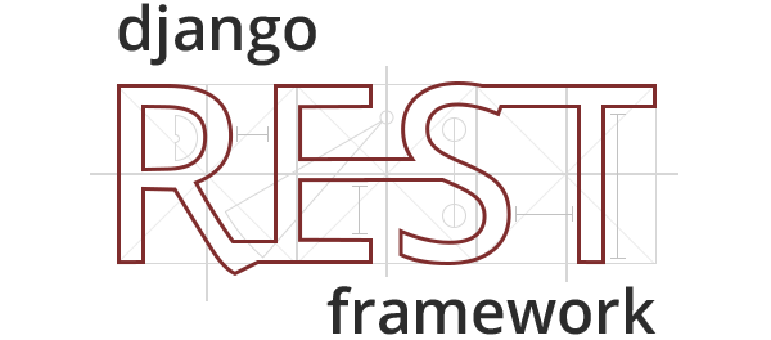
\includegraphics{images/django-rest-framework}
\caption{Logo Django REST frameworku \autocite{djangorest}\label{pic:djangorest}}
\end{figure}

\begin{figure}
\centering
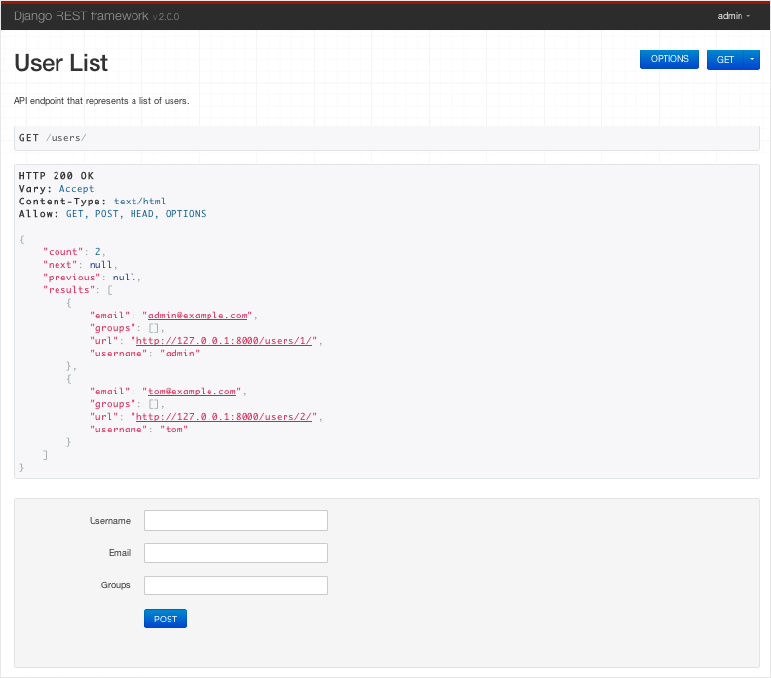
\includegraphics{images/django-rest-framework-browsable}
\caption{Django REST framework: Webově procházetelné API \autocite{djangorest}\label{pic:djangorestbrowsable}}
\end{figure}

Za vývojem Django REST frameworku nestojí žádná firma, ale jednotlivec, Tom Christie. Kromě něj ale do projektu přispělo více než pět set přispěvatelů \autocite{djangorestcontributors}. Projekt navíc absolvoval crowdfundingovou kampaň a podpořilo jej mnoho firem i jednotlivců \autocite{djangorestkickstarter}. Zveřejněn je podobně jako Django pod BSD licencí \autocite{BSD2}.

Příklad použití z~dokumentace, mírně upravený, aby se vešel na stránku, najdete \protect\hyperlink{code:djangorest}{v~ukázce}.

\begin{listing}[htbp]
\caption{{\label{code:djangorest}Příklad použití z~dokumentace Django REST frameworku \autocite{djangorestdoc}}}
\begin{minted}[bgcolor=codebg]{python}
# Serializers
from django.contrib.auth.models import User, Group
from rest_framework import serializers

class UserSerializer(serializers.HyperlinkedModelSerializer):
    class Meta:
        model = User
        fields = ('url', 'username', 'email', 'groups')

class GroupSerializer(serializers.HyperlinkedModelSerializer):
    class Meta:
        model = Group
        fields = ('url', 'name')

# Views
from django.contrib.auth.models import User, Group
from rest_framework import viewsets
from tutorial.quickstart.serializers import UserSerializer
from tutorial.quickstart.serializers import GroupSerializer

class UserViewSet(viewsets.ModelViewSet):
    """
    API endpoint that allows users to be viewed or edited.
    """
    queryset = User.objects.all().order_by('-date_joined')
    serializer_class = UserSerializer

class GroupViewSet(viewsets.ModelViewSet):
    """
    API endpoint that allows groups to be viewed or edited.
    """
    queryset = Group.objects.all()
    serializer_class = GroupSerializer

# URLs
from django.conf.urls import url, include
from rest_framework import routers
from tutorial.quickstart import views

router = routers.DefaultRouter()
router.register(r'users', views.UserViewSet)
router.register(r'groups', views.GroupViewSet)

# Wire up our API using automatic URL routing.
# Additionally, we include login URLs for the browsable API.
urlpatterns = [
    url(r'^', include(router.urls)),
    url(r'^api-auth/', include('rest_framework.urls',
                               namespace='rest_framework'))
]
\end{minted}
\end{listing}

První verze byla vydána již v~roce 2011 a od té doby jich vyšlo celkem osmdesát; poslední cca tři týdny před psaním tohoto textu. Vývoj je velmi aktivní a dokumentace obsáhlá. Instalace závisí pouze na Djangu, které nemá žádné další závislosti, a společně s~ním má 79~854 řádků kódu. Podporovány jsou obě verze Pythonu. Na GitHubu má více než pět a půl tisíce hvězd a za poslední měsíc byl více než třistatisíckrát stažen z~PyPI.

\subsection{HATEOAS}\label{hateoas}

Dokumentace obsahuje kapitolu o~HATEOAS \autocite{djangoresthateoas}, která uvádí:

\begin{quote}
Je zřejmé, že (Django) REST framework umožňuje vytvářet Hypermedia API. Procházetelné API, které nabízí, je postaveno na HTML -- jazyku hypermédií webu.

(Django) REST framework také obsahuje serializační, parsovací a renderovací komponenty usnadňující vytváření patřičných mediálních typů, hyperlinkovaných vazeb pro konstrukci vysoce propojených systémů, a dobrou podporu pro vyjednávání obsahu.

Co ale (Django) REST framework neumí, je vytváření strojově čitelných formátů hypermédií jako HAL, Collection+JSON, JSON API či HTML mikroformátů ve výchozí konfiguraci, či automagické generování plně HATEOAS API s~hypermediálním popisem formulářů a sémanticky označenými hyperlinky. To by vyžadovalo provedení takových rozhodnutí o~designu API, která by ve skutečnosti měla zůstat vně pole působnosti tohoto frameworku.
\end{quote}

Hodnotím kladně, že se o~principu HATEOAS v~dokumentaci hovoří. Prolinkování zdrojů ve stylu HATEOAS je v~Django REST frameworku jednoduché. Naplnění konkrétních implementací však zůstává v~režii architekta či programátora; Django REST framework k~tomu poskytuje dostatečné možnosti, uděluji mu tedy tři body.

\subsection{Přístupová práva}\label{pux159uxedstupovuxe1-pruxe1va}

Django REST framework umožňuje jak různé způsoby autentizace \autocite{djangorestauth}, tak i autorizace \autocite{djangorestperm}. V~základu poskytuje autentizaci:

\begin{itemize}
\tightlist
\item
  uživatelským jménem a heslem,
\item
  tokenem,
\item
  pomocí session.
\end{itemize}

Zároveň je možné implementovat vlastní způsoby. Existují další Python moduly, které tuto možnost využívají a přidávají tak do Django REST frameworku další možnosti autentizace, mezi ty nejdůležitější patří moduly pro OAuth~1 i OAuth~2. Například Django REST framework OAuth je modul, který byl dříve součástí Django REST frameworku, ale nyní je spravován samostatně.

Přístupová práva je možné řešit na úrovni objektů, modelů či konkrétních pohledů, tedy vlastně na základě URL. Pro první dvě kategorie se používají zabudované mechanismy přímo z~Djanga. Jsou rozlišena práva pro čtení a pro zápis. Stejně jako u~autentizace, i zde je možné si napsat vlastní způsob rozhodování přístupových práv a i zde vzniklo několik modulů třetích stran.

Možností poskytuje mnoho, Django REST framework tedy dostává i zde tři body.

Celkově Django REST framework působí jako obsáhlý nástroj poskytující mnoho možností a funkcí. Jeho jedinou zjevnou slabinou je těsná provázanost s~Djangem.
